% Archivo generado automáticamente con los problemas
\section*{Problems}
Sección: 2_Lorentz_invariance_and_second_quantization
Páginas: 46-47
Contenido:
2.1 Derive the transformations x →
x+vt
√
1−v2 and t →
t+vx
√
1−v2 in perturbation theory. Start
with the Galilean transformation x →x + vt. Add a transformation t →t + δt and
solve for δt assuming it is linear in x and t and preserves t2−x2 to O

v2
. Repeat for
δt and δx to second order in v and show that the result agrees with the second-order
expansion of the full transformations.

2.2 Special relativity and colliders.
(a) The Large Hadron Collider was designed to collide protons together at 14 TeV
center-of-mass energy. How many kilometers per hour less than the speed of light
are the protons moving?
(b) How fast is one proton moving with respect to the other?

2.3 The GZK bound. In 1966 Greisen, Zatsepin and Kuzmin argued that we should
not see cosmic rays (high-energy protons hitting the atmosphere from outer space)
above a certain energy, due to interactions of these rays with the cosmic microwave
background.
(a) The universe is a blackbody at 2.73 K. What is the average energy of the photons
in outer space (in electronvolts)?
(b) How much energy would a proton (p+) need to collide with a photon (γ) in outer
space to convert it to a 135 MeV pion (π0)? That is, what is the energy threshold
for p+ + γ →p+ + π0?
(c) How much energy does the outgoing proton have after this reaction?
This GZK bound was finally confirmed experimentally 40 years after it was conjec-
tured [Abbasi et al., 2008].

2.4 Is the transformation Y : (t, x, y, z) →(t, x, −y, z) a Lorentz transformation? If so,
why is it not considered with P and T as a discrete Lorentz transformation? If not,
why not?

2.5 Compton scattering. Suppose we scatter an X-ray off an electron in a crystal, but we
cannot measure the electron’s momentum, just the reflected X-ray momentum.
(a) Why is it OK to treat the electrons as free?
(b) Calculate the frequency dependence of the reflected X-ray on the scattering angle.
Draw a rough plot.
(c) What happens to the distribution as you take the electron mass to zero?
28
Lorentz invariance and second quantization
(d) If you did not believe in quantized photon momenta, what kind of distribution
might you have expected? [Hint: see [Compton, 1923].]

2.6 Lorentz invariance.
(a) Show that
 ∞
−∞
dk0δ(k2 −m2)θ(k0) =
1
2ωk
,
(2.103)
where θ(x) is the unit step function and ωk ≡
⃗k2 + m2.
(b) Show that the integration measure d4k is Lorentz invariant.
(c) Finally, show that
 d3k
2ωk
(2.104)
is Lorentz invariant.

2.7 Coherent states of the simple harmonic oscillator.
(a) Calculate ∂z(e−za†aeza†) where z is a complex number.
(b) Show that |z⟩= eza†|0⟩is an eigenstate of a. What is its eigenvalue?
(c) Calculate ⟨n|z⟩.
(d) Show that these “coherent states” are minimally dispersive: ΔpΔq = 1
2, where
Δq2 = ⟨q2⟩−⟨q⟩2 and Δp2 = ⟨p2⟩−⟨p⟩2, where ⟨q⟩= ⟨z|q|z⟩
⟨z|z⟩and ⟨p⟩= ⟨z|p|z⟩
⟨z|z⟩.
(e) Why can you not make an eigenstate of a†?

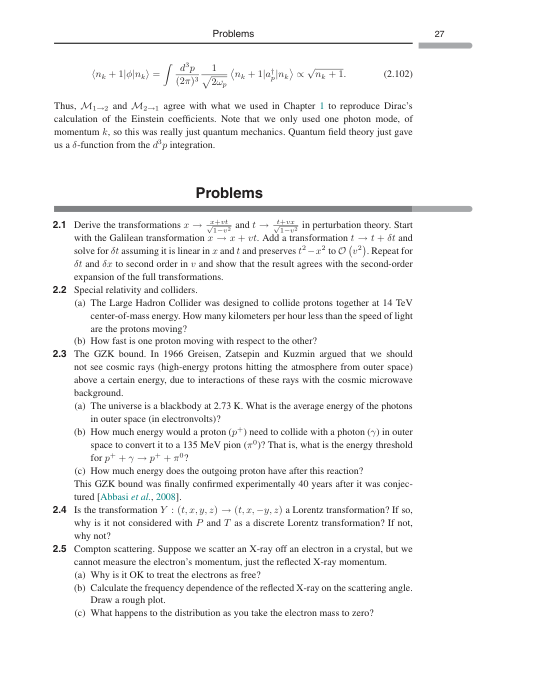
\includegraphics{./figs/2_Lorentz_invariance_and_second_quantization_page_47.png}

---

